\subsection{Park Generation}
The ParkGenerator, much like the BuildingGenerator, has the primary task of filling city plots with visually pleasing, interesting content. 
To accomplish this, the ParkGenerator was implemented as a function that takes two inputs, the plot to generate the park in and the underlying terrain.
These parameters are then used to produce a park as output (see Table~\ref{table:parkgen}).

Since real-world parks come in all sizes and shapes, and can contain a variety of different objects, a scope had to be defined for what to include in the parks for this project.
For the scope of this project, the objects were limited to bushes, trees, rocks, and paths, but it was implemented in such a way that it would be simple to add more objects such as benches, fountains, and statues.

\begin{table}[H]
   \centering
   \begin{tabular}{lllll}
     \textbf{Input}                           &               & \textbf{Function}            &               & \textbf{Output}         \\
     \midrule
     \textit{Plot, Terrain}                   & $\rightarrow$ & \textbf{ParkGenerator}       & $\rightarrow$ & \textit{Park}           \\
     \bottomrule
   \end{tabular}

   \caption{Definition of the ParkGenerator function which is responsible for generating parks.}
   \label{table:parkgen}
 \end{table}
 \vspace{-0.4cm}
 
The development of the Park Generator consisted of two main phases:
\begin{easylist}
 @ Filling the park with objects such as trees, bushes, and rocks.
 @ Creating natural paths for people to walk on.
\end{easylist}
To make the parks vary in appearance through procedural generation, a way to randomize the placement of objects inside any given plot had to be constructed.
However, pure randomness of placement would produce some unrealistic results.
Another problem to tackle was the frequency of objects i.e. determining how much of each object is reasonable to have within each park. 
For example, one tree, 43 stones, and two bushes would likely look like an odd park.
 
The algorithm for generating objects was implemented by making use of uniform randomness between 0 and 10.
The range 0-10 was split into several separate, but not equally large sub-ranges, which would determine what object to generate.
For example numbers in the range [6,10] could result in a tree, [2,5] could result in a bush, and [0,1] could result in a rock.
As real-world objects are never identical, having one model for each object type would not be sufficient. 
Therefore, once the object type is decided, a model is sampled from an array of such model types, and then randomly rotated and scaled. 

It was considered important to be able to distinguish the park-objects based on size and type as these parameters would determine how far from each other objects would be allowed to be generated.
This is referred to as giving each object-type a radius relative to other object-types.
A function was then constructed to search within the radius of each object and make sure no object could be created within another object's radius (see Figure~\ref{fig:radius}).
This implementation is based on Poisson Disc Sampling \cite{poisson_fast} in a manner that it scatters points randomly across the plot, while maintaining a distance from each already created point.
Here the object-radius is used in order to determine how closely objects may stack. 
When the paths were implemented, a slight adjustment also had to be made to the algorithm for object placement, such that all objects took into consideration the coordinates of the path and were not placed on top of it.
\begin{figure}[H]
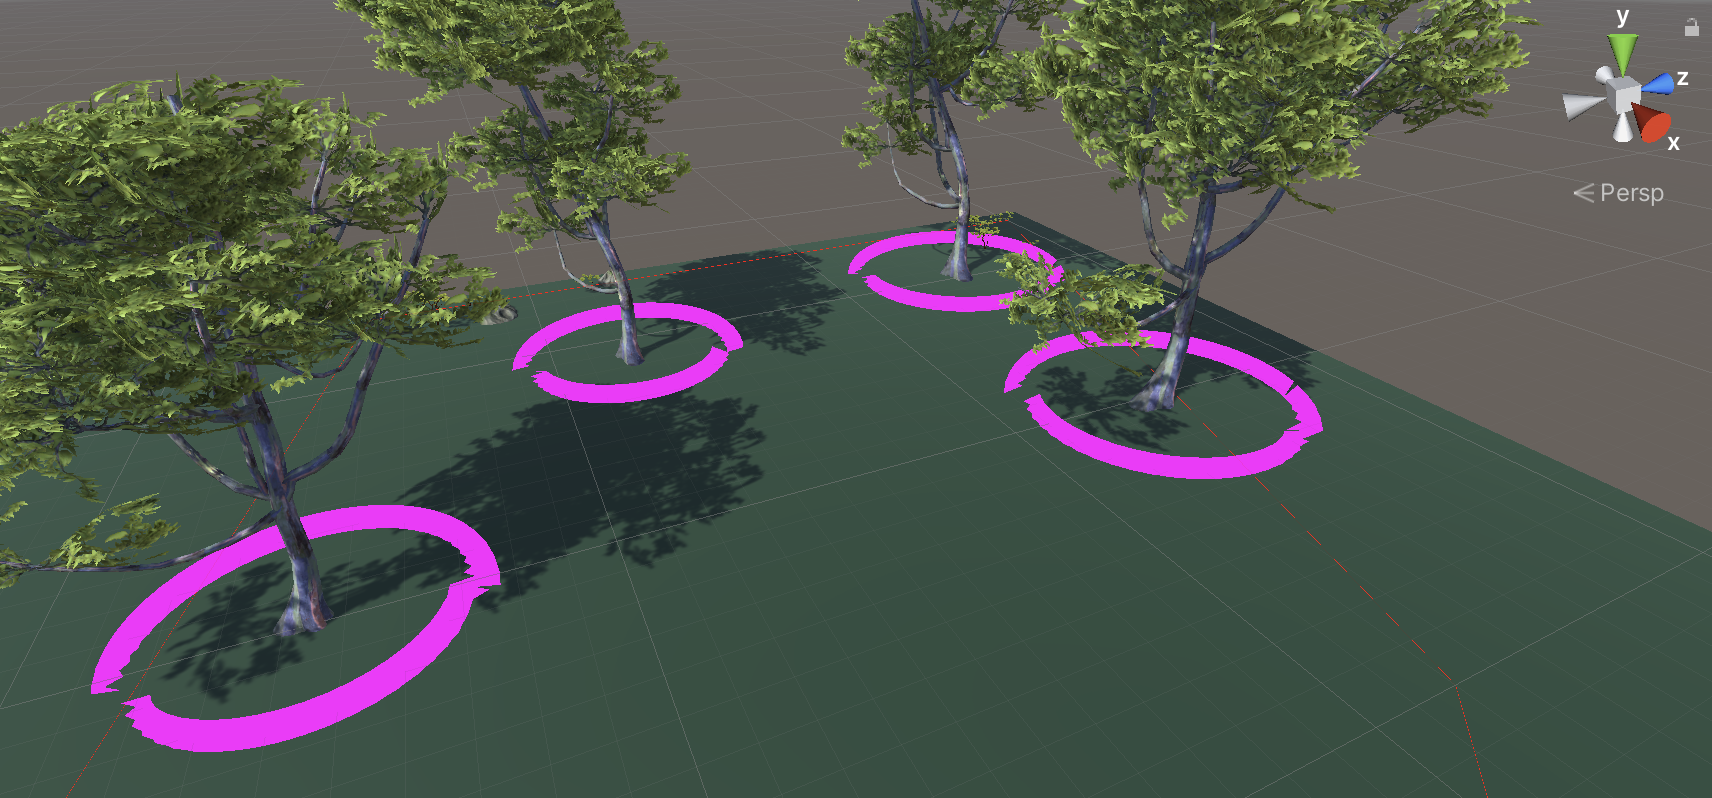
\includegraphics[width=\linewidth]{figure/radiuscontrol.png}
\caption{Radius of the tree object shown in pink. This radius indicates how closely trees may pack.}
\label{fig:radius}
\end{figure}

The algorithm for creating paths was inspired by Cyclic Dungeon Generation \cite{cyclic}.
The main takeaway from that concept was that a start and goal node was generated for the algorithm to create a loop between.
Having a loop would allow for people to take a stroll around the park and return to where they entered, and based on observation, this is also a frequently occurring pattern for paths in real-world parks. 

The development of the path generation can be described as three iterations of implementation.
The first implementation of the algorithm created two random points within the plot, one as start and another one as goal. 
The program then traveled the park at random until it found a path to the goal, at which point it would find a new way back to the starting point. 
It was however, quickly discovered that this approach had some problems.
 
One of these problems were that the paths would look unnatural when taking steps far away from the goal. 
A solution to this was to revert the path to its previous node if it took a step which was further away from the goal than it had previously been, this was an instant improvement in appearance. 
However, after observing many of the generated paths from this approach the paths still looked linear. 
This was believed to be because simply going from one point to another and not straying off too much from the goal could not produce much more interesting results than that (see Figure~\ref{fig:linear}).
\begin{figure}[H]
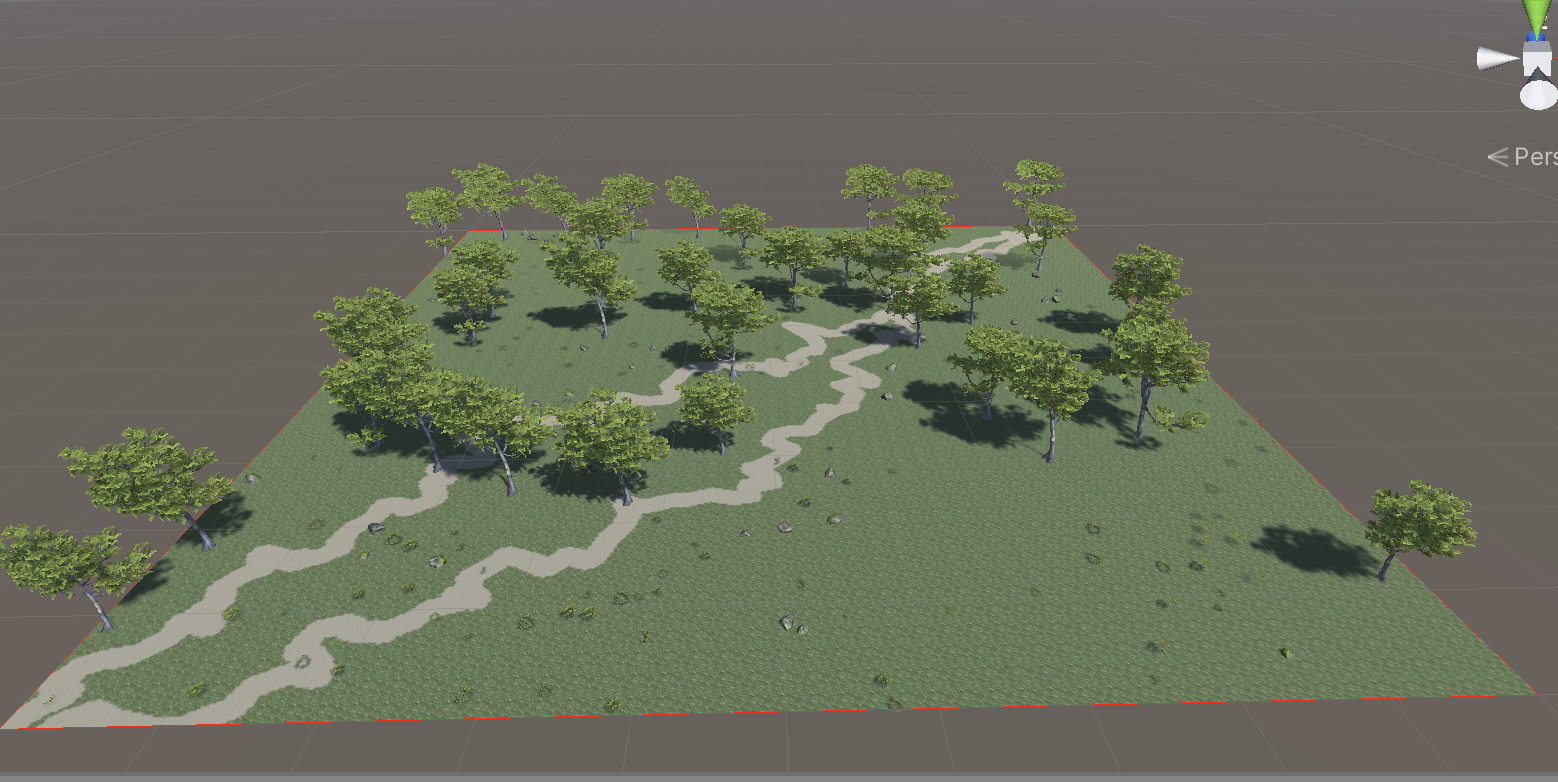
\includegraphics[width=\linewidth]{figure/linear.png}
\caption{Example of a path generated by the first implementation of the algorithm.}
\label{fig:linear}
\end{figure}
The second implementation of the algorithm was inspired by the flaws which had been demonstrated by its predecessor, more specifically its linear shapes and its tendency to create steps with abrupt angle-changes.
As a result of this, it was for the second implementation decided that rather than having a start and goal, the path would consist of an array of points, which all had to be visited before the path would be completed.
This was changed in order to try to get rid off the linearity presented in the first implementation.
For this implementation a control of how many degrees a step in the path could differ from the current point to its previous step was also added.
This was done to avoid the zigzag-like patterns caused by the angle-changes from the first implementation.
The second implementation would just like the first one look for one assigned point, but in this case start searching for the next point after finding the previous one and continue doing so until all points have been found (see Figure~\ref{fig:texsplat}). 
\begin{figure}[H]
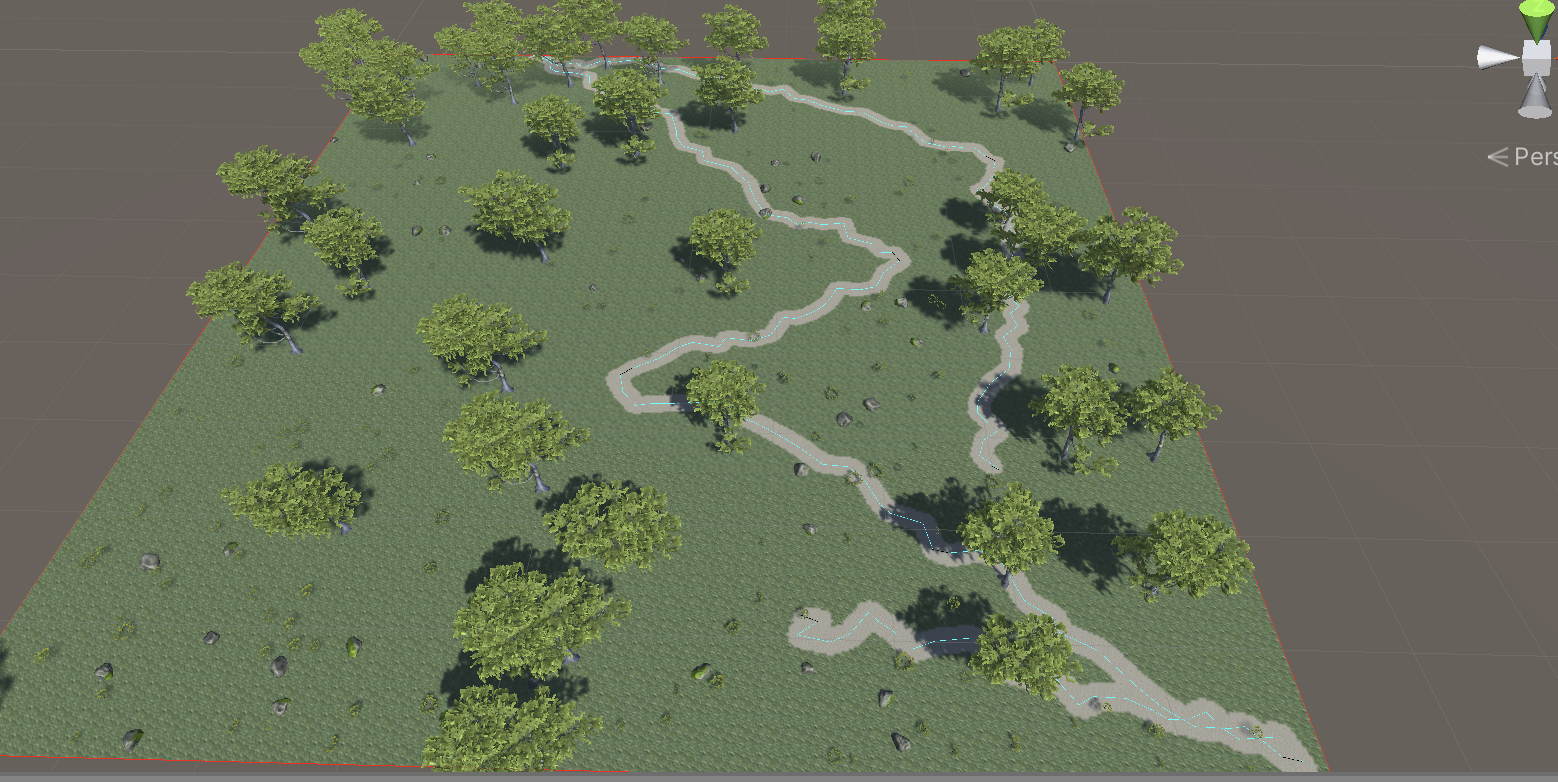
\includegraphics[width=\linewidth]{figure/texturesplat}
\caption{Example of a path generated by the second implementation of the algorithm.}
\label{fig:texsplat}
\end{figure}
The third and final implementation made use of a similar algorithm.
Some fairly small changes were made in order to address the issues experienced with the second implementation.
The second implementation would still create paths starting in the middle of the park which did not make a lot of sense, this was handled by always creating the start node on one of the edges of the plot.
The algorithm then creates an additional number of randomly placed points, based on the size of the plot.
Having this number be based on the size of the plot made for some more interesting and realistic results which was lacking in the second implementation.

Afterwards, the points are sorted by distance to enforce that the algorithm always traverses towards the point closest to itself. 
This change was inspired by seeing some paths traverse towards points far away from the starting point only to then traverse to a point close to the starting point.
Once all goal points have been reached a path is either created back to the starting node, or a new path is created to a randomly selected edge on the plot. 
This change was made to stop enforcing loops and to add more variety to the generated paths.
Finally, the algorithm creates entries to the park by projecting a line to closest edge of the plot from some of the points, and then creating a path between them. 
 
The visual implementation of the paths was done by texture splatting on top of a Unity Terrain for the first two implementations (see Figure~\ref{fig:linear} and Figure~\ref{fig:texsplat}).
However, as the Unity Terrain needed to be replaced with a mesh generated one, this had to be re-implemented for the third implementation.
Some different approaches for visualizing the paths were investigated, such as using quad and sphere meshes and then simply placing these along each path.
The spheres would cause a shape that was still distinguishably circular and the quads would likewise create patterns that were clearly square. 
The final implementation would instead make use of the logic from the RoadGenerator to create its own internal road network, thereby inheriting the functionality used to generate the corresponding path mesh (see Figure~\ref{fig:visuals}).
\begin{figure}[H]
  \centering
  \begin{subfigure}[b]{0.4\textwidth}
    \frame{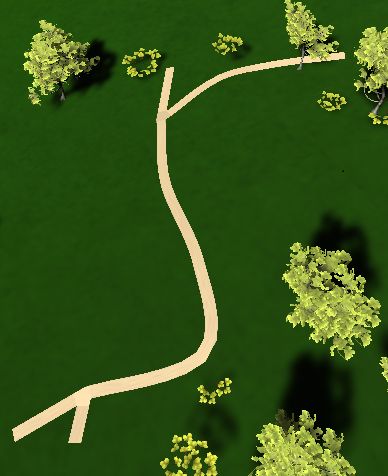
\includegraphics[width=\textwidth]{figure/pathvisualized}}
    \caption{Visualization of a path using splines.}
  \end{subfigure}
  \quad
  \begin{subfigure}[b]{0.35\textwidth}
    \frame{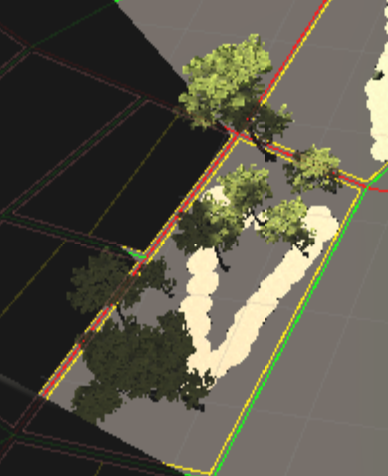
\includegraphics[width=\textwidth]{figure/spherepath}}
    \caption{Visualization of a path using spheres.}
  \end{subfigure}
  \caption{Two of the approaches for visualizing paths on top of the mesh generated terrain.}
  \label{fig:visuals}
\end{figure}
